\documentclass{standalone}

\usepackage{tikz}

\begin{document}

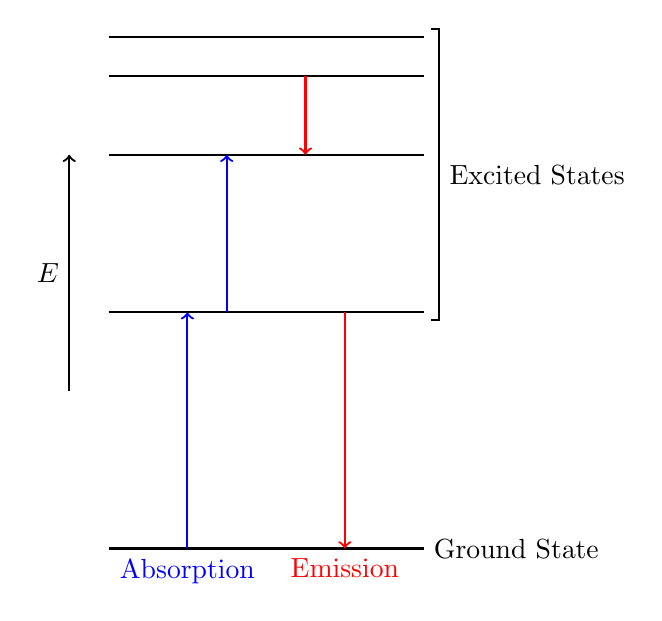
\begin{tikzpicture}[every path/.style={thick}]
	\draw (0,0) -- (4,0) node[right] {Ground State};
	\draw (0,3) -- (4,3);
	\draw (0,5) -- (4,5);
	\draw (0,6) -- (4,6);
	\draw (0,6.5) -- (4,6.5);
	\draw[->,blue] (1,0) -- (1,3) node[pos=0,below] {Absorption};
	\draw[->,blue] (1.5,3) -- (1.5,5);
	\draw[->,red] (2.5,6) -- (2.5,5);
	\draw[->,red] (3,3) -- (3,0) node[pos=1,below] {Emission};
	\draw (4.1,6.6) -- (4.2,6.6) -- (4.2,2.9) node[midway,right] {Excited
	States} -- (4.1,2.9);
	\draw[->] (-0.5,2) -- (-0.5,5) node[midway,left] {$E$};
\end{tikzpicture}

\end{document}
